\section{Inverse Trigonometric Functions}

\label{ArcTrig}

As the title indicates, in this section we concern ourselves with finding inverses of the (circular) trigonometric functions.  Our immediate problem is that, owing to their periodic nature, none of the six circular functions is  one-to-one. To remedy this, we restrict the domains of the circular functions in the same way we restricted the domain of the quadratic function in Example \ref{inverserestrictionex} in Section \ref{InverseFunctions} to obtain a one-to-one function.  We first consider $f(x) = \cos(x)$. Choosing the interval $[0,\pi]$ allows us to keep the range as $[-1,1]$ as well as the properties of being smooth and continuous.

\medskip

\noindent\begin{minipage}{\textwidth}
\begin{center}
\myincludegraphics[width=\textwidth]{figures/IntroTrigGraphics/ArcTrig-1}
\end{center} 
\captionsetup{type=figure}
\caption{Restricting the domain of $f(x) = \cos(x)$ to $[0,\pi]$.}
\label{fig:arctrig1}
\end{minipage}

\medskip

Recall from Section \ref{InverseFunctions} that the inverse of a function $f$ is typically denoted $f^{-1}$.  For this reason, some textbooks use the notation $f^{-1}(x) = \cos^{-1}(x)$ for the inverse of $f(x) = \cos(x)$.  The obvious pitfall here is our convention of writing $(\cos(x))^2$ as $\cos^{2}(x)$, $(\cos(x))^3$ as $\cos^{3}(x)$ and so on.  It is far too easy to confuse $\cos^{-1}(x)$ with  $\frac{1}{\cos(x)} = \sec(x)$ so we will not use this notation in our text. (But be aware that many books do! As always, be sure to check the context!) Instead, we use the notation $f^{-1}(x) = \arccos(x)$, read `arc-cosine of $x$'.  To understand the `arc' in `arccosine', recall that an inverse function, by definition, reverses the process of the original function. The function $f(t) = \cos(t)$ takes a real number input $t$, associates it with the angle $\theta = t$ radians, and returns the value $\cos(\theta)$.  Digging deeper,  we have that $\cos(\theta) = \cos(t)$ is the $x$-coordinate of the terminal point on the Unit Circle of an oriented arc of length $|t|$ whose initial point is $(1, 0)$.  Hence, we may view the inputs to $f(t) = \cos(t)$ as oriented arcs and the outputs as $x$-coordinates on the Unit Circle.  The function $f^{-1}$, then, would take $x$-coordinates on the Unit Circle and return oriented arcs, hence the `arc' in arccosine. Figure \ref{fig:arctrig2} shows the graphs of $f(x) = \cos(x)$ and $f^{-1}(x) = \arccos(x)$, where we obtain the latter from the former by reflecting it across the line $y=x$, in accordance with Theorem \ref{inverseuniquegraph}. \index{arccosine ! graph of}

%\mnote{.5}{See page \pageref{wrappingfunction} if you need a review of how we associate real numbers with angles in radian measure.}
\mtable{.4}{Reflecting $y=\cos(x)$ across $y=x$ yields $y=\arccos(x)$}{fig:arctrig2}{
\begin{tabular}{c}
\myincludegraphics[width=0.95\marginparwidth]{figures/IntroTrigGraphics/ArcTrig-2}\\
$f(x) = \cos(x)$, $0 \leq x \leq \pi$\\
\\
\myincludegraphics[width=0.95\marginparwidth]{figures/IntroTrigGraphics/ArcTrig-3}\\
$f^{-1}(x) = \arccos(x)$
\end{tabular}}

We restrict $g(x) = \sin(x)$ in a similar manner, although the interval of choice is $\left[ -\frac{\pi}{2}, \frac{\pi}{2}\right]$.

\medskip

\noindent\begin{minipage}{\textwidth}
\begin{center}
\myincludegraphics[width=\textwidth]{figures/IntroTrigGraphics/ArcTrig-4}
\end{center}
\captionsetup{type=figure}
\caption{Restricting the domain of $f(x) = \sin(x)$ to $\left[-\frac{\pi}{2}, \frac{\pi}{2}\right]$.}
\label{fig:arctrig3}
\end{minipage}

\medskip

It should be no surprise that we call $g^{-1}(x) = \arcsin(x)$, which is read `arc-sine of $x$'. \index{arcsine ! graph of}


We list some important facts about the arccosine and arcsine functions in the following theorem. 

\smallskip

\theorem{arccosinesinefunctionprops}{Properties of the Arccosine and Arcsine Functions}{\index{arccosine ! definition of} \index{arccosine ! properties of} \index{arcsine ! definition of} \index{arcsine ! properties of} 

\begin{itemize}

\item  Properties of $F(x)= \arccos(x)$

\begin{itemize}

\item Domain:  $[-1,1]$

\item Range:  $[0,\pi]$

\item $\arccos(x) = t$ if and only if $0 \leq t \leq \pi$ and $\cos(t) = x$

\item $\cos(\arccos(x)) = x$ provided $-1 \leq x \leq 1$

\item $\arccos(\cos(x)) = x$ provided $0 \leq x \leq \pi$

\end{itemize}

\item  Properties of $G(x) = \arcsin(x)$

\begin{itemize}

\item Domain:  $[-1,1]$

\item Range:  $\left[ -\frac{\pi}{2}, \frac{\pi}{2}\right]$

\item $\arcsin(x) = t$ if and only if $-\frac{\pi}{2} \leq t \leq \frac{\pi}{2}$ and $\sin(t) = x$

\item $\sin(\arcsin(x)) = x$ provided $-1 \leq x \leq 1$

\item $\arcsin(\sin(x)) = x$ provided $-\frac{\pi}{2} \leq x \leq \frac{\pi}{2}$ 

\item additionally, arcsine is odd

\end{itemize}

\end{itemize}
}

\mtable{.7}{Reflecting $y=\sin(x)$ across $y=x$ yields $y=\arcsin(x)$}{fig:arctrig4}{
\begin{tabular}{c}
\myincludegraphics[width=0.95\marginparwidth]{figures/IntroTrigGraphics/ArcTrig-5}\\
$g(x) = \sin(x)$,  $-\frac{\pi}{2} \leq x \leq  \frac{\pi}{2}$\\
\\
\myincludegraphics[width=0.95\marginparwidth]{figures/IntroTrigGraphics/ArcTrig-6}\\
$g^{-1}(x) = \arcsin(x)$
\end{tabular}}


Everything in Theorem \ref{arccosinesinefunctionprops} is a direct consequence of the facts that $f(x) = \cos(x)$ for $0 \leq x \leq \pi$ and $F(x) = \arccos(x)$ are inverses of each other as are $g(x) = \sin(x)$ for $-\frac{\pi}{2} \leq x \leq \frac{\pi}{2}$ and $G(x) = \arcsin(x)$.  It's about time for an example.



\medskip

\example{arccosinesineex}{Evaluating the arcsine and arccosine functions}{

\begin{enumerate}  

\item Find the exact values of the following.

\begin{multicols}{2}

\begin{enumerate}

\item  $\arccos\left(\frac{1}{2}\right)$ 
\item  $\arcsin\left(\frac{\sqrt{2}}{2}\right)$
\item  $\arccos\left(-\frac{\sqrt{2}}{2}\right)$
\item  $\arcsin\left(-\frac{1}{2}\right)$
\item  $\arccos\left( \cos\left(\frac{\pi}{6}\right)\right)$
\item  $\arccos\left( \cos\left(\frac{11\pi}{6}\right)\right)$
\item  $\cos\left(\arccos\left(-\frac{3}{5}\right)\right)$
\item  $\sin\left(\arccos\left(-\frac{3}{5}\right)\right)$

\end{enumerate}

\end{multicols}

\item  \label{algarcsincos} Rewrite the following as algebraic expressions of $x$ and state the domain on which the equivalence is valid.

\begin{multicols}{2}

\begin{enumerate}

\item \label{tanarccos} $\tan\left(\arccos\left(x \right)\right)$

\item  \label{cosarcsin} $\cos\left(2 \arcsin(x)\right)$

\end{enumerate}

\end{multicols}

\end{enumerate}}
{
\begin{enumerate}

\item 

\begin{enumerate}

\item  To find $\arccos\left(\frac{1}{2}\right)$, we need to find the real number $t$ (or, equivalently, an angle measuring $t$ radians) which lies between $0$ and $\pi$ with $\cos(t) = \frac{1}{2}$. We know $t = \frac{\pi}{3}$ meets these criteria, so $\arccos\left(\frac{1}{2}\right)= \frac{\pi}{3}$.

\item  The value of $\arcsin\left(\frac{\sqrt{2}}{2}\right)$ is a real number $t$ between $-\frac{\pi}{2}$ and $\frac{\pi}{2}$ with $\sin(t) = \frac{\sqrt{2}}{2}$.  The number we seek is  $t = \frac{\pi}{4}$. Hence, $\arcsin\left(\frac{\sqrt{2}}{2}\right) = \frac{\pi}{4}$.

\item  The number $t = \arccos\left(-\frac{\sqrt{2}}{2}\right)$ lies in the interval $[0,\pi]$ with $\cos(t) = -\frac{\sqrt{2}}{2}$.  Our answer is $\arccos\left(-\frac{\sqrt{2}}{2}\right) = \frac{3\pi}{4}$.

\item  To find  $\arcsin\left(-\frac{1}{2}\right)$, we seek the number $t$ in the interval $\left[-\frac{\pi}{2}, \frac{\pi}{2}\right]$ with $\sin(t) = -\frac{1}{2}$.  The answer is $t = -\frac{\pi}{6}$ so that $\arcsin\left(-\frac{1}{2}\right) = -\frac{\pi}{6}$.

\item  Since $0 \leq \frac{\pi}{6} \leq \pi$, one option would be to simply invoke Theorem \ref{arccosinesinefunctionprops} to get $\arccos\left( \cos\left(\frac{\pi}{6}\right)\right) = \frac{\pi}{6}$.  However, in order to make sure we understand \textit{why} this is the case, we choose to work the example through using the definition of arccosine.  Working from the inside out,  $\arccos\left( \cos\left(\frac{\pi}{6}\right)\right) = \arccos\left( \frac{\sqrt{3}}{2}\right)$.  Now, $\arccos\left( \frac{\sqrt{3}}{2}\right)$ is the real number $t$ with $0 \leq t \leq \pi$ and $\cos(t) = \frac{\sqrt{3}}{2}$.  We find $t = \frac{\pi}{6}$, so that  $\arccos\left( \cos\left(\frac{\pi}{6}\right)\right) = \frac{\pi}{6}$.

\item Since $\frac{11\pi}{6}$ does not fall between $0$ and $\pi$, Theorem \ref{arccosinesinefunctionprops} does not apply.  We are forced to work through from the inside out starting with  $\arccos\left( \cos\left(\frac{11\pi}{6}\right)\right) = \arccos\left(\frac{\sqrt{3}}{2}\right)$.  From the previous problem, we know $\arccos\left(\frac{\sqrt{3}}{2}\right) = \frac{\pi}{6}$.  Hence,  $\arccos\left( \cos\left(\frac{11\pi}{6}\right)\right) = \frac{\pi}{6}$.

\item  One way to simplify  $\cos\left(\arccos\left(-\frac{3}{5}\right)\right)$ is to use Theorem \ref{arccosinesinefunctionprops} directly.  Since $-\frac{3}{5}$ is between $-1$ and $1$, we have that $\cos\left(\arccos\left(-\frac{3}{5}\right)\right) = -\frac{3}{5}$ and we are done.  However, as before, to really understand \textit{why} this cancellation occurs, we  let $t = \arccos\left(-\frac{3}{5}\right)$.  Then, by definition,  $\cos(t) = -\frac{3}{5}$. Hence, $\cos\left(\arccos\left(-\frac{3}{5}\right)\right) = \cos(t) = -\frac{3}{5}$, and we are finished in (nearly) the same amount of time.

\item  As in the previous example, we let $t = \arccos\left(-\frac{3}{5}\right)$ so that  $\cos(t) = -\frac{3}{5}$ for some $t$ where  $0 \leq t \leq \pi$.  Since $\cos(t) < 0$, we can narrow this down a bit and conclude that $\frac{\pi}{2} < t < \pi$, so that $t$ corresponds to an angle in Quadrant II. In terms of $t$, then, we need to find $\sin\left(\arccos\left(-\frac{3}{5}\right)\right) = \sin(t)$.  Using the Pythagorean Identity $\cos^{2}(t) + \sin^{2}(t) = 1$, we get $\left(-\frac{3}{5}\right)^2 + \sin^{2}(t) = 1$ or $\sin(t) = \pm \frac{4}{5}$.  Since $t$ corresponds to a Quadrants II angle, we choose  $\sin(t) = \frac{4}{5}$.  Hence,  $\sin\left(\arccos\left(-\frac{3}{5}\right)\right) = \frac{4}{5}$.

\end{enumerate}

\drawexampleline

\item

\begin{enumerate}

\mnote{.2}{An alternative approach to finding $\tan(t)$ is to use the identity  $1 + \tan^{2}(t) = \sec^{2}(t)$.  Since $x = \cos(t)$,  $\sec(t) = \frac{1}{\cos(t)} = \frac{1}{x}$.  The reader is invited to work through this approach to see what, if any, difficulties arise.}

\item We begin this problem in the same manner we began the previous two problems.  To help us see the forest for the trees, we let  $t = \arccos(x)$, so our goal is to find a way to express $\tan\left(\arccos\left(x \right)\right) = \tan(t)$ in terms of $x$.  Since $t = \arccos(x)$, we know $\cos(t) = x$ where $0 \leq t \leq \pi$, but since we are after an expression for $\tan(t)$, we know we need to throw out $t = \frac{\pi}{2}$ from consideration.  Hence, either $0 \leq t < \frac{\pi}{2}$ or $\frac{\pi}{2} < t \leq \pi$ so that, geometrically, $t$ corresponds to an angle in Quadrant I or Quadrant II.  One approach to finding $\tan(t)$ is to use the quotient identity $\tan(t) = \frac{\sin(t)}{\cos(t)}$.   Substituting $\cos(t) = x$ into the Pythagorean Identity $\cos^{2}(t) + \sin^{2}(t) = 1$ gives $x^2 + \sin^{2}(t) = 1$, from which we get $\sin(t) = \pm \sqrt{1-x^2}$.  Since $t$ corresponds to angles in Quadrants I and II,   $\sin(t) \geq 0$, so we choose $\sin(t) = \sqrt{1-x^2}$.  Thus, \[\tan(t) = \dfrac{\sin(t)}{\cos(t)} = \dfrac{\sqrt{1-x^2}}{x}\]  To determine the values of $x$ for which this equivalence is valid, we consider our substitution $t = \arccos(x)$.  Since the domain of $\arccos(x)$ is $[-1,1]$, we know we must restrict $-1 \leq x \leq 1$.  Additionally, since we had to discard $t = \frac{\pi}{2}$, we need to discard $x = \cos\left(\frac{\pi}{2}\right) = 0$. Hence, $\tan\left(\arccos\left(x \right)\right) =\frac{\sqrt{1-x^2}}{x}$  is valid for $x$ in $[-1,0)\cup(0,1]$.

\item We proceed as in the previous problem by writing $t = \arcsin(x)$ so that $t$ lies in the interval $\left[ -\frac{\pi}{2}, \frac{\pi}{2}\right]$ with $\sin(t) = x$.  We aim to express $\cos\left(2 \arcsin(x)\right) = \cos(2t)$ in terms of $x$.  Since $\cos(2t)$ is defined everywhere, we get no additional restrictions on $t$ as we did in the previous problem.  We have three choices for rewriting $\cos(2t)$:  $\cos^{2}(t) - \sin^{2}(t)$, $2\cos^{2}(t) - 1$ and $1 - 2\sin^{2}(t)$.  Since we know $x = \sin(t)$, it is easiest to use the last form: \[\cos\left(2 \arcsin(x)\right) = \cos(2t)  = 1 - 2\sin^{2}(t) = 1 - 2x^2\]  To find the restrictions on $x$, we once again appeal to our substitution $t = \arcsin(x)$.  Since $\arcsin(x)$ is defined only for $-1 \leq x \leq 1$, the equivalence $\cos\left(2 \arcsin(x)\right) = 1-2x^2$ is valid only on $[-1,1]$. 

\end{enumerate}

\end{enumerate}
}

\medskip

A few remarks about Example \ref{arccosinesineex} are in order.  Most of the common errors encountered in dealing with the inverse circular functions come from the need to restrict the domains of the original functions so that they are one-to-one.  One instance of this phenomenon is the fact that $\arccos\left( \cos\left(\frac{11\pi}{6}\right)\right) = \frac{\pi}{6}$ as opposed to $\frac{11\pi}{6}$. This is the exact same phenomenon discussed in Section \ref{InverseFunctions} when we saw  $\sqrt{(-2)^2} = 2$ as opposed to $-2$.    Additionally, even though the expression we arrived at in part \ref{cosarcsin} above, namely $1 - 2x^2$, is defined for all real numbers, the equivalence  $\cos\left(2 \arcsin(x)\right) = 1-2x^2$ is valid for only $-1 \leq x \leq 1$.  This is akin to the fact that while the expression $x$ is defined for all real numbers, the equivalence $\left( \sqrt{x} \right)^2 = x$ is valid only for $x \geq 0$.  For this reason, it pays to be careful when we determine the intervals where such equivalences are valid.



\bigskip

The next pair of functions we wish to discuss are the inverses of tangent and cotangent, which are named arctangent and arccotangent, respectively.  First, we restrict $f(x) = \tan(x)$ to its fundamental cycle on $\left(-\frac{\pi}{2}, \frac{\pi}{2}\right)$ to obtain $f^{-1}(x) = \arctan(x)$. Among other things, note that the \textit{vertical} asymptotes $x = -\frac{\pi}{2}$ and $x = \frac{\pi}{2}$ of the graph of $f(x) = \tan(x)$ become the \textit{horizontal} asymptotes $y = -\frac{\pi}{2}$ and $y = \frac{\pi}{2}$ of the graph of $f^{-1}(x) = \arctan(x)$: see Figure \ref{fig:arctrig5}.  \index{arctangent ! graph of}

\mtable{.3}{Reflecting $y=\tan(x)$ across $y=x$ yields $y=\arctan(x)$}{fig:arctrig5}{ 
\begin{tabular}{c}
\myincludegraphics[width=0.6\marginparwidth]{figures/IntroTrigGraphics/ArcTrig-7}\\
$f(x) = \tan(x)$,  $-\frac{\pi}{2} < x <  \frac{\pi}{2}$\\
\\
\myincludegraphics[width=0.95\marginparwidth]{figures/IntroTrigGraphics/ArcTrig-8}\\
$f^{-1}(x) = \arctan(x)$
\end{tabular}}


Next, we restrict $g(x) = \cot(x)$ to its fundamental cycle on $(0,\pi)$ to obtain $g^{-1}(x) = \operatorname{arccot}(x)$.  Once again, the vertical asymptotes $x=0$ and $x=\pi$ of the graph of $g(x) = \cot(x)$ become the horizontal asymptotes $y = 0$ and $y = \pi$ of the graph of $g^{-1}(x) = \operatorname{arccot}(x)$.  We show these graphs in Figure \ref{fig:arctrig5a}; \index{arccotangent ! graph of}
the basic properties of the arctangent and arccotangent functions are given in the following theorem.

\smallskip

\theorem{arctangentcotangentfunctionprops}{Properties of the Arctangent and Arccotangent Functions}{ \index{arctangent ! definition of} \index{arctangent ! properties of} \index{arccotangent ! definition of} \index{arccotangent ! properties of} 

\begin{itemize}

\item Properties of $F(x)= \arctan(x)$

\begin{itemize}

\item Domain: $(-\infty, \infty)$

\item Range: $\left(-\frac{\pi}{2}, \frac{\pi}{2}\right)$

\item  as $x \rightarrow -\infty$, $\arctan(x) \rightarrow -\frac{\pi}{2}^{+}$;  as $x \rightarrow \infty$, $\arctan(x) \rightarrow \frac{\pi}{2}^{-}$

\item  $\arctan(x) = t$ if and only if $-\frac{\pi}{2} < t < \frac{\pi}{2}$ and $\tan(t) = x$

\item  $\arctan(x) = \operatorname{arccot}\left(\frac{1}{x}\right)$ for $x > 0$

\item  $\tan\left(\arctan(x)\right) = x$ for all real numbers $x$

\item  $\arctan(\tan(x)) = x$ provided $-\frac{\pi}{2} < x < \frac{\pi}{2}$

\item additionally, arctangent is odd

\end{itemize}

\item Properties of $G(x) = \operatorname{arccot}(x)$

\begin{itemize}

\item Domain: $(-\infty, \infty)$

\item Range: $(0, \pi)$

\item  as $x \rightarrow -\infty$, $\operatorname{arccot}(x) \rightarrow \pi^{-}$; as $x \rightarrow \infty$, $\operatorname{arccot}(x) \rightarrow 0^{+}$

\item  $\operatorname{arccot}(x) = t$ if and only if $0 <  t < \pi$ and $\cot(t) = x$

\item  $\operatorname{arccot}(x) =\arctan\left(\frac{1}{x}\right)$ for $x > 0$

\item  $\cot\left(\operatorname{arccot}(x)\right) = x$ for all real numbers $x$

\item  $\operatorname{arccot}(\cot(x)) = x$ provided $0 < x < \pi$

\end{itemize}

\end{itemize}
}

\mtable{.7}{Reflecting $y=\cot(x)$ across $y=x$ yields $y=\operatorname{arccot}(x)$}{fig:arctrig5a}{ 
\begin{tabular}{c}
\myincludegraphics[width=0.75\marginparwidth]{figures/IntroTrigGraphics/ArcTrig-9}\\
$g(x) = \cot(x)$,  $0 < x <  \pi$\\
\\
\myincludegraphics[width=0.95\marginparwidth]{figures/IntroTrigGraphics/ArcTrig-10}\\
$gf^{-1}(x) = \operatorname{arccot}(x)$
\end{tabular}}

\medskip

\example{ex_arctan}{Evaluating the arctangent and arccotangent functions}{

\begin{enumerate}

\item  Find the exact values of the following.

\begin{multicols}{2}

\begin{enumerate}

\item $\arctan(\sqrt{3})$
\item  $\operatorname{arccot}(-\sqrt{3})$

\setcounter{HW}{\value{enumii}}

\end{enumerate}

\end{multicols}

\begin{multicols}{2}

\begin{enumerate}

\setcounter{enumii}{\value{HW}}

\item  $\cot(\operatorname{arccot}(-5))$
\item  $\sin\left(\arctan\left(-\frac{3}{4}\right)\right)$

\end{enumerate}

\end{multicols}

\item  Rewrite the following as algebraic expressions of $x$ and state the domain on which the equivalence is valid.

\begin{multicols}{2}

\begin{enumerate}

\item  $\tan(2 \arctan(x))$

\item  $\cos(\operatorname{arccot}(2x))$ 

\end{enumerate}

\end{multicols}

\end{enumerate}
}
{
\begin{enumerate}

\item

\begin{enumerate}

\item  We know $\arctan(\sqrt{3})$ is the real number $t$ between $-\frac{\pi}{2}$ and $\frac{\pi}{2}$ with $\tan(t) = \sqrt{3}$.  We find $t = \frac{\pi}{3}$, so $\arctan(\sqrt{3}) = \frac{\pi}{3}$.

\item The real number $t = \operatorname{arccot}(-\sqrt{3})$ lies in the interval $(0,\pi)$ with $\cot(t) = -\sqrt{3}$.  We get $\operatorname{arccot}(-\sqrt{3}) = \frac{5\pi}{6}$.

\item  We can apply Theorem \ref{arctangentcotangentfunctionprops} directly and obtain $\cot(\operatorname{arccot}(-5)) = -5$.  However, working it through provides us with yet another opportunity to understand why this is the case. Letting $t = \operatorname{arccot}(-5)$, we have that $t$ belongs to the interval $(0,\pi)$ and $\cot(t)=-5$.  Hence, $\cot(\operatorname{arccot}(-5)) = \cot(t)=-5$.

\item   We start simplifying  $\sin\left(\arctan\left(-\frac{3}{4}\right)\right)$ by letting $t = \arctan\left(-\frac{3}{4}\right)$.  Then $\tan(t) = -\frac{3}{4}$ for some $-\frac{\pi}{2} < t < \frac{\pi}{2}$.  Since $\tan(t) < 0$, we know, in fact, $-\frac{\pi}{2} < t < 0$.  One way to proceed is to use The Pythagorean Identity, $1 + \cot^{2}(t) = \csc^{2}(t)$, since this relates the reciprocals of $\tan(t)$ and $\sin(t)$ and is valid for all $t$ under consideration.   From  $\tan(t) = -\frac{3}{4}$, we get $\cot(t) = -\frac{4}{3}$.  Substituting, we get $1 + \left(-\frac{4}{3}\right)^2 = \csc^{2}(t)$ so that $\csc(t) = \pm \frac{5}{3}$.  Since $-\frac{\pi}{2} < t < 0$, we choose $\csc(t) = -\frac{5}{3}$, so $\sin(t) = -\frac{3}{5}$. Hence, $\sin\left(\arctan\left(-\frac{3}{4}\right)\right) = -\frac{3}{5}$.

\end{enumerate}

\enlargethispage{2\baselineskip}

\mnote{.5}{It's always a good idea to make sure the identities used in these situations are valid for all values $t$ under consideration.  Check our work back in Example \ref{arccosinesineex}.  Were the identities we used there valid for all $t$ under consideration?  A pedantic point, to be sure, but what else do you expect from this book?}

\item  

\begin{enumerate}

\item If we let $t = \arctan(x)$, then $-\frac{\pi}{2} < t < \frac{\pi}{2}$ and $\tan(t) = x$.   We look for a way to express $\tan(2 \arctan(x)) = \tan(2t)$ in terms of $x$.  Before we get started using identities, we note that $\tan(2t)$ is undefined when $2t = \frac{\pi}{2} + \pi k$ for integers $k$.  Dividing both sides of this equation by $2$ tells us we need to exclude values of $t$ where $t = \frac{\pi}{4} + \frac{\pi}{2} k$, where $k$ is an integer.  The only members of this family which lie in $\left(-\frac{\pi}{2}, \frac{\pi}{2}\right)$ are $t = \pm \frac{\pi}{4}$, which means the values of $t$ under consideration are $\left(-\frac{\pi}{2}, -\frac{\pi}{4}\right) \cup \left(-\frac{\pi}{4}, \frac{\pi}{4}\right) \cup \left(\frac{\pi}{4}, \frac{\pi}{2}\right)$.  Returning to $\arctan(2t)$, we note the double angle identity $\tan(2t) = \frac{2 \tan(t)}{1 - \tan^{2}(t)}$, is valid for all the values of $t$ under consideration, hence we get \[\tan(2 \arctan(x)) = \tan(2t) = \frac{2 \tan(t)}{1 - \tan^{2}(t)}= \frac{2x}{1-x^2}\]  To find where this equivalence is valid we check back with our substitution $t = \arctan(x)$. Since the domain of $\arctan(x)$ is all real numbers, the only exclusions come from the values of $t$ we discarded earlier, $t = \pm \frac{\pi}{4}$.   Since $x =\tan(t)$, this means we exclude $x = \tan\left(\pm \frac{\pi}{4}\right) = \pm 1$.  Hence, the equivalence  $\tan(2 \arctan(x)) =  \frac{2x}{1-x^2}$ holds for all $x$ in  $(-\infty, -1) \cup (-1,1) \cup (1,\infty)$.

\item  To get started, we let $t = \operatorname{arccot}(2x)$ so that  $\cot(t) = 2x$ where $0 < t < \pi$.  In terms of $t$, $\cos(\operatorname{arccot}(2x)) = \cos(t)$, and our goal is to express the latter in terms of $x$.   Since $\cos(t)$ is always defined, there are no additional restrictions on $t$, so we can begin using identities to relate $\cot(t)$ to $\cos(t)$.  The identity $\cot(t) = \frac{\cos(t)}{\sin(t)}$ is valid for $t$ in $(0,\pi)$, so our strategy is to obtain $\sin(t)$ in terms of $x$, then write $\cos(t) = \cot(t) \sin(t)$.   The identity $1 + \cot^{2}(t) = \csc^{2}(t)$ holds for all $t$ in $(0,\pi)$ and relates $\cot(t)$ and $\csc(t) = \frac{1}{\sin(t)}$.  Substituting $\cot(t) =2x$, we get  $1 + (2x)^2 = \csc^{2}(t)$, or $\csc(t) =  \pm \sqrt{4x^2+1}$. Since $t$ is between $0$ and $\pi$, $\csc(t) > 0$, so $\csc(t) =\sqrt{4x^2+1}$ which gives $\sin(t) = \frac{1}{\sqrt{4x^2+1}}$. Hence, \[\cos(\operatorname{arccot}(2x)) = \cos(t) = \cot(t) \sin(t) = \frac{2x}{\sqrt{4x^2+1}}\]   Since $\operatorname{arccot}(2x)$ is defined for all real numbers $x$ and we encountered no additional restrictions on $t$, we have  $\cos\left(\operatorname{arccot}(2x)\right) = \frac{2x}{\sqrt{4x^2+1}}$ for all real numbers $x$. 

\end{enumerate}

\end{enumerate}
}

\pagebreak



The last two functions to invert are secant and cosecant.  A portion of each of their graphs, which were first discussed in Subsection \ref{secantcosecantgraphsection}, are given in Figure \ref{fig:arctrig6} below with the fundamental cycles highlighted. 

\bigskip

\noindent\begin{minipage}{\textwidth}
\begin{center}
\begin{tabular}{cc}
\myincludegraphics[width=0.45\textwidth]{figures/IntroTrigGraphics/ArcTrig-11} & \myincludegraphics[width=0.45\textwidth]{figures/IntroTrigGraphics/ArcTrig-12}\\
The graph $y=\sec(x)$ & The graph $y=\csc(x)$
\end{tabular}
\end{center}
\captionsetup{type=figure}
\caption{The fundamental cycles of $f(x)=\sec(x)$ and $g(x)=\csc(x)$}
\label{fig:arctrig6}
\end{minipage}

\bigskip

It is clear from the graph of secant that we cannot find one single continuous piece of its graph which covers its entire range of $(-\infty, -1] \cup [1, \infty)$ and restricts the domain of the function so that it is one-to-one.  The same is true for cosecant.  Thus in order to define the arcsecant and arccosecant functions, we must settle for a piecewise approach wherein we choose one piece to cover the top of the range, namely  $[1, \infty)$, and another piece to cover the bottom, namely $(-\infty, -1]$.  There are two generally accepted ways make these choices which restrict the domains of these functions so that they are one-to-one.  One approach simplifies the Trigonometry associated with the inverse functions, but complicates the Calculus;  the other makes the Calculus easier, but the Trigonometry less so.  We present both points of view.

%\newpage

\subsection{Inverses of Secant and Cosecant: Trigonometry Friendly Approach}

In this subsection, we restrict the secant and cosecant functions to coincide with the restrictions on cosine and sine, respectively.  For $f(x) = \sec(x)$, we restrict the domain to $\left[0, \frac{\pi}{2}\right) \cup \left( \frac{\pi}{2}, \pi\right]$ (Figure \ref{fig:arctrig7}) \index{arcsecant ! trigonometry friendly ! graph of} and we restrict $g(x) = \csc(x)$ to $\left[-\frac{\pi}{2}, 0\right) \cup \left(0,  \frac{\pi}{2}\right]$ (Figure \ref{fig:arctrig8}. \index{arccosecant ! trigonometry friendly ! graph of}


Note that for both arcsecant and arccosecant, the domain is $(-\infty, -1] \cup [1, \infty)$.  Taking a page from Section \ref{AbsoluteValueFunctions}, we can rewrite this as $\left\{ x : |x| \geq 1\right\}$.  This is often done in Calculus textbooks, so we include it here for completeness.  Using these definitions, we get the following properties of the arcsecant and arccosecant functions.

\smallskip

\theorem{arcsecantcosecantfunctionprops1}{Properties of the Arcsecant and Arccosecant Functions (``Trigonometry Friendly'' version)}{ 

\begin{itemize}

\item Properties of $F(x)= \operatorname{arcsec}(x)$ \index{arcsecant ! trigonometry friendly ! definition of} \index{arcsecant ! trigonometry friendly ! properties of}

\begin{itemize}

\item Domain:  $\left\{ x : |x| \geq 1 \right\} = (-\infty, -1] \cup [1,\infty)$

\item Range:  $\left[0, \frac{\pi}{2} \right) \cup \left(\frac{\pi}{2}, \pi\right]$

\item  as $x \rightarrow -\infty$, $\operatorname{arcsec}(x) \rightarrow \frac{\pi}{2}^{+}$;  as $x \rightarrow \infty$, $\operatorname{arcsec}(x) \rightarrow \frac{\pi}{2}^{-}$

\item  $\operatorname{arcsec}(x) = t$ if and only if $0 \leq t < \frac{\pi}{2}$ or $ \frac{\pi}{2} < t \leq \pi$ and $\sec(t) = x$

\item  $\operatorname{arcsec}(x) = \arccos\left(\frac{1}{x}\right)$ provided $|x| \geq 1$

\item  $\sec\left(\operatorname{arcsec}(x)\right) = x$ provided $|x| \geq 1$

\item  $\operatorname{arcsec}(\sec(x)) = x$ provided $0 \leq x < \frac{\pi}{2}$ or $\frac{\pi}{2} < x \leq \pi$

\end{itemize}

\item  Properties of $G(x) = \operatorname{arccsc}(x)$ \index{arccosecant ! trigonometry friendly ! definition of} \index{arccosecant ! trigonometry friendly ! properties of}

\begin{itemize}

\item  Domain:  $\left\{ x : |x| \geq 1 \right\} = (-\infty, -1] \cup [1,\infty)$

\item Range:  $\left[-\frac{\pi}{2}, 0 \right) \cup \left(0, \frac{\pi}{2} \right]$

\item  as $x \rightarrow -\infty$, $\operatorname{arccsc}(x) \rightarrow 0^{-}$;  as $x \rightarrow \infty$, $\operatorname{arccsc}(x) \rightarrow 0^{+}$

\item  $\operatorname{arccsc}(x) = t$ if and only if $-\frac{\pi}{2} \leq t < 0$ or $0 < t \leq \frac{\pi}{2}$ and $\csc(t) = x$

\item  $\operatorname{arccsc}(x) = \arcsin\left(\frac{1}{x}\right)$ provided $|x| \geq 1$

\item  $\csc\left(\operatorname{arccsc}(x)\right) = x$ provided $|x| \geq 1$

\item  $\operatorname{arccsc}(\csc(x)) = x$ provided $-\frac{\pi}{2} \leq x < 0$ or $0 < x \leq \frac{\pi}{2}$

\item additionally, arccosecant is odd

\end{itemize}

\end{itemize}
}

\medskip

\mtable{.7}{The ``Trigonometry Friendly'' definition of $\operatorname{arcsec}(x)$}{fig:arctrig7}{
\begin{tabular}{c}
\myincludegraphics[width=0.7\marginparwidth]{figures/IntroTrigGraphics/ArcTrig-13}\\
$f(x) = \sec(x)$ on  $\left[0, \frac{\pi}{2}\right) \cup \left( \frac{\pi}{2}, \pi\right]$\\
\\
\myincludegraphics[width=0.9\marginparwidth]{figures/IntroTrigGraphics/ArcTrig-14}\\
$f^{-1}(x)=\operatorname{arcsec}(x)$
\end{tabular}}
 

\mtable{.3}{The ``Trigonometry Friendly'' definition of $\operatorname{arccsc}(x)$}{fig:arctrig8}{
\begin{tabular}{c}
\myincludegraphics[width=0.7\marginparwidth]{figures/IntroTrigGraphics/ArcTrig-15}\\
$g(x) = \csc(x)$ on  $\left[-\frac{\pi}{2}, 0\right) \cup \left(0,  \frac{\pi}{2}\right]$\\
\\
\myincludegraphics[width=0.9\marginparwidth]{figures/IntroTrigGraphics/ArcTrig-16}\\
$g^{-1}(x)=\operatorname{arccsc}(x)$
\end{tabular}}


\example{arcsecantcosecantex1}{Evaluating the arcsecant and arccosecant functions}{

\begin{enumerate}

\item  Find the exact values of the following.

\begin{multicols}{2}

\begin{enumerate}

\item $\operatorname{arcsec}(2)$

\item  $\operatorname{arccsc}(-2)$

\item  $\operatorname{arcsec}\left( \sec\left( \frac{5\pi}{4} \right) \right)$

\item  $\cot\left(\operatorname{arccsc}\left(-3\right)\right)$

\end{enumerate}

\end{multicols}

\item  Rewrite the following as algebraic expressions of $x$ and state the domain on which the equivalence is valid.

\begin{multicols}{2}

\begin{enumerate}

\item  $\tan(\operatorname{arcsec}(x))$

\item  $\cos(\operatorname{arccsc}(4x))$ 

\end{enumerate}

\end{multicols}

\end{enumerate}
}
{
\begin{enumerate}

\item

\begin{enumerate}

\item Using Theorem \ref{arcsecantcosecantfunctionprops1}, we have $\operatorname{arcsec}(2) = \arccos\left(\frac{1}{2}\right) = \frac{\pi}{3}$.

\item  Once again, Theorem \ref{arcsecantcosecantfunctionprops1} gives us $\operatorname{arccsc}(-2) = \arcsin\left(-\frac{1}{2}\right) = -\frac{\pi}{6}$.


\item  Since $\frac{5\pi}{4}$ doesn't fall between $0$ and $\frac{\pi}{2}$ or $\frac{\pi}{2}$ and $\pi$, we cannot use the inverse property stated in Theorem \ref{arcsecantcosecantfunctionprops1}.  We can, nevertheless, begin by working `inside out' which yields  $\operatorname{arcsec}\left( \sec\left( \frac{5\pi}{4} \right) \right) = \operatorname{arcsec}(-\sqrt{2}) = \arccos\left(-\frac{\sqrt{2}}{2}\right) = \frac{3\pi}{4}$.

\item   One way to begin to simplify $\cot\left(\operatorname{arccsc}\left(-3\right)\right)$ is to let $t = \operatorname{arccsc}(-3)$.  Then,  $\csc(t) = -3$ and, since this is negative, we have that $t$ lies in the interval  $\left[ -\frac{\pi}{2},0\right)$.  We are after $\cot\left(\operatorname{arccsc}\left(-3\right)\right) = \cot(t)$, so we use the Pythagorean Identity $1 + \cot^{2}(t) = \csc^{2}(t)$.  Substituting, we have $1 + \cot^{2}(t) = (-3)^2$, or $\cot(t) = \pm \sqrt{8} = \pm 2 \sqrt{2}$.  Since $-\frac{\pi}{2} \leq t < 0$, $\cot(t) < 0$, so we get  $\cot\left(\operatorname{arccsc}\left(-3\right)\right) = -2\sqrt{2}$.

\end{enumerate}

\item 

\begin{enumerate}


\item  We begin simplifying  $\tan(\operatorname{arcsec}(x))$ by letting $t = \operatorname{arcsec}(x)$.  Then, $\sec(t) = x$ for $t$ in $\left[0, \frac{\pi}{2}\right) \cup \left(\frac{\pi}{2}, \pi \right]$, and we seek a formula for $\tan(t)$.  Since $\tan(t)$ is defined for all $t$ values under consideration, we have no additional restrictions on $t$.  To relate $\sec(t)$ to $\tan(t)$, we use the identity $1 + \tan^{2}(t) = \sec^{2}(t)$.  This is valid for all values of $t$ under consideration, and when we substitute $\sec(t) = x$, we get $1 + \tan^{2}(t) = x^2$.  Hence, $\tan(t) = \pm \sqrt{x^2-1}$.  If $t$ belongs to $\left[0, \frac{\pi}{2}\right)$ then $\tan(t) \geq 0$;  if, on the the other hand, $t$ belongs to  $\left(\frac{\pi}{2}, \pi \right]$ then $\tan(t) \leq 0$. As a result, we get a piecewise defined function for $\tan(t)$

\[ 
\tan(t) = \left\{\begin{array}{rr} \sqrt{x^2-1}, & \text{ if } 0 \leq t < \frac{\pi}{2} \\ [5pt] -\sqrt{x^2-1}, & \text{ if } \frac{\pi}{2} < t \leq \pi  \end{array}\right. 
\]

Now we need to determine what these conditions on $t$ mean for $x$.  Since $x = \sec(t)$, when $0 \leq t < \frac{\pi}{2}$, $x \geq 1$, and when $\frac{\pi}{2} < t \leq \pi$, $x \leq -1$.  Since we encountered no further restrictions on $t$, the  equivalence below holds for all $x$ in $(-\infty, -1] \cup [1, \infty)$.

\[ \tan(\operatorname{arcsec}(x)) = \left\{ \begin{array}{rr} \sqrt{x^2-1}, & \text{if $x \geq 1$} \\[5pt]  -\sqrt{x^2-1}, & \text{if $x \leq -1$}  \end{array}\right. \]



\item  To simplify $\cos(\operatorname{arccsc}(4x))$, we start by letting $t = \operatorname{arccsc}(4x)$.   Then $\csc(t) = 4x$ for $t$ in $\left[-\frac{\pi}{2}, 0 \right) \cup \left(0, \frac{\pi}{2}\right]$, and we now set about finding an expression for  $\cos(\operatorname{arccsc}(4x)) = \cos(t)$.  Since $\cos(t)$ is defined for all $t$, we do not encounter any additional restrictions on $t$.  From $\csc(t) = 4x$, we get $\sin(t) = \frac{1}{4x}$, so to find $\cos(t)$, we can make use if the identity $\cos^{2}(t) + \sin^{2}(t) = 1$.  Substituting $\sin(t) = \frac{1}{4x}$  gives $\cos^{2}(t) + \left(\frac{1}{4x}\right)^2 = 1$.  Solving, we get \[\cos(t) = \pm \sqrt{\frac{16x^2-1}{16x^2}} = \pm \frac{\sqrt{16x^2-1}}{4|x|}\]  Since $t$ belongs to $\left[-\frac{\pi}{2}, 0 \right) \cup \left(0, \frac{\pi}{2}\right]$, we know $\cos(t) \geq 0$, so we choose $\cos(t) = \frac{\sqrt{16-x^2}}{4|x|}$. (The absolute values here are necessary, since $x$ could be negative.)  To find the values for which this equivalence is valid, we look back at our original substution,  $t = \operatorname{arccsc}(4x)$.  Since the domain of $\operatorname{arccsc}(x)$ requires its argument $x$ to satisfy $|x| \geq 1$, the domain of $\operatorname{arccsc}(4x)$ requires $|4x| \geq 1$.  Using Theorem \ref{absolutevalueineq}, we rewrite this inequality and solve to get $x \leq -\frac{1}{4}$ or $x \geq \frac{1}{4}$.  Since we had no additional restrictions on $t$, the equivalence  $\cos(\operatorname{arccsc}(4x)) = \frac{\sqrt{16x^2-1}}{4|x|}$  holds for all $x$ in $\left(-\infty, -\frac{1}{4} \right] \cup \left[\frac{1}{4}, \infty \right)$.  

\end{enumerate}

\end{enumerate}
}

\medskip



\subsection{Inverses of Secant and Cosecant: Calculus Friendly Approach}

In this subsection, we restrict $f(x) = \sec(x)$ to $\left[0, \frac{\pi}{2}\right) \cup \left[\pi, \frac{3\pi}{2}\right)$, \index{arcsecant ! calculus friendly ! graph of} and we restrict $g(x) = \csc(x)$ to $\left(0, \frac{\pi}{2}\right] \cup \left( \pi, \frac{3\pi}{2}\right]$.  \index{arccosecant ! calculus friendly ! graph of}


Using these definitions, we get the following result.

\smallskip

\theorem{arcsecantcosecantfunctionprops2}{Properties of the Arcsecant and Arccosecant Functions (``Calculus Friendly'' version)}{  

\begin{itemize}

\item Properties of $F(x)= \operatorname{arcsec}(x)$ \index{arcsecant ! calculus friendly ! definition of} \index{arcsecant ! calculus friendly ! properties of}

\begin{itemize}

\item Domain: $\left\{ x : |x| \geq 1 \right\} = (-\infty, -1] \cup [1,\infty)$

\item Range: $\left[0, \frac{\pi}{2} \right) \cup \left[\pi, \frac{3\pi}{2} \right)$

\item  as $x \rightarrow -\infty$, $\operatorname{arcsec}(x) \rightarrow \frac{3\pi}{2}^{-}$;  as $x \rightarrow \infty$, $\operatorname{arcsec}(x) \rightarrow \frac{\pi}{2}^{-}$

\item  $\operatorname{arcsec}(x) = t$ if and only if $0 \leq t < \frac{\pi}{2}$ or $ \pi \leq  t < \frac{3\pi}{2}$ and $\sec(t) = x$

\item  $\operatorname{arcsec}(x) = \arccos\left(\frac{1}{x}\right)$ for $x \geq 1$ only (Compare this with the similar result in Theorem \ref{arcsecantcosecantfunctionprops1}.)

\item  $\sec\left(\operatorname{arcsec}(x)\right) = x$ provided $|x| \geq 1$

\item  $\operatorname{arcsec}(\sec(x)) = x$ provided $0 \leq x < \frac{\pi}{2}$ or $ \pi \leq  x < \frac{3\pi}{2}$


\end{itemize}

\item Properties of $G(x) = \operatorname{arccsc}(x)$ \index{arccosecant ! calculus friendly ! definition of} \index{arccosecant ! calculus friendly ! properties of}

\begin{itemize}

\item Domain: $\left\{ x : |x| \geq 1 \right\} = (-\infty, -1] \cup [1,\infty)$

\item Range: $\left(0, \frac{\pi}{2} \right] \cup \left( \pi, \frac{3\pi}{2} \right]$

\item  as $x \rightarrow -\infty$, $\operatorname{arccsc}(x) \rightarrow \pi^{+}$;  as $x \rightarrow \infty$, $\operatorname{arccsc}(x) \rightarrow 0^{+}$

\item  $\operatorname{arccsc}(x) = t$ if and only if $0 < t \leq \frac{\pi}{2}$ or $\pi < t \leq \frac{3\pi}{2}$ and $\csc(t) = x$

\item  $\operatorname{arccsc}(x) = \arcsin\left(\frac{1}{x}\right)$ for $x \geq 1$ only (Compare this with the similar result in Theorem \ref{arcsecantcosecantfunctionprops1}.)

\item  $\csc\left(\operatorname{arccsc}(x)\right) = x$ provided $|x| \geq 1$

\item  $\operatorname{arccsc}(\csc(x)) = x$ provided $0 < x \leq \frac{\pi}{2}$ or $\pi < x \leq \frac{3\pi}{2}$

\end{itemize}

\end{itemize}
}

\medskip


\mtable{.71}{The ``Calculus Friendly'' definition of $\operatorname{arcsec}(x)$}{fig:arctrig9}{
\begin{tabular}{c}
\myincludegraphics[width=0.8\marginparwidth]{figures/IntroTrigGraphics/ArcTrig-17}\\
$f(x) = \sec(x)$ on  $\left[0, \frac{\pi}{2}\right) \cup \left[ \pi, \frac{3\pi}{2}\right)$\\
\\
\myincludegraphics[width=0.9\marginparwidth]{figures/IntroTrigGraphics/ArcTrig-18}\\
$f^{-1}(x)=\operatorname{arcsec}(x)$
\end{tabular}}
 

\mtable{.28}{The ``Calculus Friendly definition of $\operatorname{arccsc}(x)$}{fig:arctrig10}{
\begin{tabular}{c}
\myincludegraphics[width=0.8\marginparwidth]{figures/IntroTrigGraphics/ArcTrig-19}\\
$g(x) = \csc(x)$ on  $\left(0, \frac{\pi}{2}\right] \cup \left(\pi,  \frac{3\pi}{2}\right]$\\
\\
\myincludegraphics[width=0.9\marginparwidth]{figures/IntroTrigGraphics/ArcTrig-20}\\
$g^{-1}(x)=\operatorname{arccsc}(x)$
\end{tabular}}

Our next example is a duplicate of Example \ref{arcsecantcosecantex1}.  The interested reader is invited to compare and contrast the solution to each.

\medskip

\example{arcsecantcosecantex2}{Evaluating the arcsecant and arccosecant functions}{

\begin{enumerate}

\item  Find the exact values of the following.

\begin{multicols}{2}

\begin{enumerate}

\item $\operatorname{arcsec}(2)$

\item  $\operatorname{arccsc}(-2)$

\item  $\operatorname{arcsec}\left( \sec\left( \frac{5\pi}{4} \right) \right)$

\item  $\cot\left(\operatorname{arccsc}\left(-3\right)\right)$

\end{enumerate}

\end{multicols}

%\enlargethispage{.25in}

\item  Rewrite the following as algebraic expressions of $x$ and state the domain on which the equivalence is valid.

\begin{multicols}{2}

\begin{enumerate}

\item  $\tan(\operatorname{arcsec}(x))$

\item  $\cos(\operatorname{arccsc}(4x))$ 

\end{enumerate}

\end{multicols}

\end{enumerate}
}
{
\begin{enumerate}
\item
\begin{enumerate}

\item  Since $2 \geq 1$, we can use Theorem \ref{arcsecantcosecantfunctionprops2} to get $\operatorname{arcsec}(2) = \arccos\left(\frac{1}{2}\right) = \frac{\pi}{3}$.

\item  Unfortunately, $-2$ is not greater to or equal to $1$, so we cannot apply Theorem \ref{arcsecantcosecantfunctionprops2} to  $\operatorname{arccsc}(-2)$ and convert this into an arcsine problem.  Instead, we appeal to the definition.  The real number $t = \operatorname{arccsc}(-2)$ lies in $\left(0,\frac{\pi}{2} \right] \cup \left(\pi, \frac{3\pi}{2}\right]$ and satisfies $\csc(t) = -2$.  The $t$ we're after is $t = \frac{7\pi}{6}$, so $\operatorname{arccsc}(-2) = \frac{7\pi}{6}$.

\item  Since $\frac{5\pi}{4}$ lies between $\pi$ and $\frac{3\pi}{2}$, we may apply Theorem \ref{arcsecantcosecantfunctionprops2} directly to simplify $\operatorname{arcsec}\left( \sec\left( \frac{5\pi}{4} \right) \right) = \frac{5\pi}{4}$.  We encourage the reader to work this through using the definition as we have done in the  previous examples to see how it goes.

\item  To help simplify $\cot\left(\operatorname{arccsc}\left(-3\right)\right)$ we define $t = \operatorname{arccsc}\left(-3\right)$ so that  $\cot\left(\operatorname{arccsc}\left(-3\right)\right) = \cot(t)$.  We know $\csc(t) = -3$, and since this is negative,  $t$ lies in $\left( \pi, \frac{3\pi}{2}\right]$.  Using the identity $1 + \cot^{2}(t) = \csc^{2}(t)$, we find $1 + \cot^{2}(t) = (-3)^2$ so that $\cot(t) = \pm \sqrt{8} = \pm 2 \sqrt{2}$.  Since $t$ is in the interval $\left(\pi, \frac{3\pi}{2}\right]$, we know $\cot(t) > 0$.  Our answer is $\cot\left(\operatorname{arccsc}\left(-3\right)\right) = 2 \sqrt{2}$.

\end{enumerate}

\drawexampleline

\item 
\begin{enumerate}

\item  We begin simplifying  $\tan(\operatorname{arcsec}(x))$ by letting $t = \operatorname{arcsec}(x)$.  Then, $\sec(t) = x$ for $t$ in $\left[0, \frac{\pi}{2} \right) \cup \left[\pi, \frac{3\pi}{2} \right)$, and we seek a formula for $\tan(t)$.  Since $\tan(t)$ is defined for all $t$ values under consideration, we have no additional restrictions on $t$.  To relate $\sec(t)$ to $\tan(t)$, we use the identity $1 + \tan^{2}(t) = \sec^{2}(t)$.  This is valid for all values of $t$ under consideration, and when we substitute $\sec(t) = x$, we get $1 + \tan^{2}(t) = x^2$.  Hence, $\tan(t) = \pm \sqrt{x^2-1}$. Since $t$ lies in $\left[0, \frac{\pi}{2} \right) \cup \left[\pi, \frac{3\pi}{2} \right)$, $\tan(t) \geq 0$, so we choose $\tan(t) = \sqrt{x^2-1}$.  Since we found no additional restrictions on $t$, the equivalence $\tan(\operatorname{arcsec}(x)) = \sqrt{x^2-1}$ holds for all $x$ in the domain of $t = \operatorname{arcsec}(x)$, namely $(-\infty, -1] \cup [1,\infty)$.

\item To simplify $\cos(\operatorname{arccsc}(4x))$, we start by letting $t = \operatorname{arccsc}(4x)$.   Then $\csc(t) = 4x$ for $t$ in $\left(0, \frac{\pi}{2} \right] \cup \left(\pi, \frac{3\pi}{2} \right]$, and we now set about finding an expression for  $\cos(\operatorname{arccsc}(4x)) = \cos(t)$.  Since $\cos(t)$ is defined for all $t$, we do not encounter any additional restrictions on $t$.  From $\csc(t) = 4x$, we get $\sin(t) = \frac{1}{4x}$, so to find $\cos(t)$, we can make use if the identity $\cos^{2}(t) + \sin^{2}(t) = 1$.  Substituting $\sin(t) = \frac{1}{4x}$  gives $\cos^{2}(t) + \left(\frac{1}{4x}\right)^2 = 1$.  Solving, we get \[\cos(t) = \pm \sqrt{\frac{16x^2-1}{16x^2}} = \pm \frac{\sqrt{16x^2-1}}{4|x|}\]  If $t$ lies in $\left(0, \frac{\pi}{2} \right]$, then $\cos(t) \geq 0$, and we choose  $\cos(t) = \frac{\sqrt{16x^2-1}}{4|x|}$. Otherwise, $t$ belongs to $\left( \pi, \frac{3\pi}{2} \right]$ in which case $\cos(t) \leq 0$, so, we choose $\cos(t) = -\frac{\sqrt{16x^2-1}}{4|x|}$ This leads us to a (momentarily) piecewise defined function for $\cos(t)$

\[ 
\cos(t) = \left\{ \begin{array}{rr}
			 \dfrac{\sqrt{16x^2-1}}{4|x|}, & \text{if $0 \leq t \leq \frac{\pi}{2}$} \\ [10pt]
			   -\dfrac{\sqrt{16x^2-1}}{4|x|}, & \text{if $\pi < t \leq \frac{3\pi}{2}$}  
			    \end{array}\right. 
\]

We now see what these restrictions mean in terms of $x$.  Since $4x = \csc(t)$, we get that for $0 \leq t \leq \frac{\pi}{2}$, $4x \geq 1$, or $x \geq \frac{1}{4}$.  In this case, we can simplify $|x| = x$ so 
\[
\cos(t) = \frac{\sqrt{16x^2-1}}{4|x|} = \frac{\sqrt{16x^2-1}}{4x}
\]  
Similarly, for $\pi < t \leq \frac{3\pi}{2}$, we get $4x \leq -1$, or $x \leq -\frac{1}{4}$.  In this case, $|x| = -x$, so we also get 
\[
\cos(t) = -\frac{\sqrt{16x^2-1}}{4|x|}  = -\frac{\sqrt{16x^2-1}}{4(-x)} =  \frac{\sqrt{16x^2-1}}{4x}
\]  
Hence, in all cases, $\cos(\operatorname{arccsc}(4x)) =  \frac{\sqrt{16x^2-1}}{4x}$, and this equivalence is valid for all $x$ in the domain of $t = \operatorname{arccsc}(4x)$, namely \\$\left(-\infty, -\frac{1}{4}\right] \cup \left[ \frac{1}{4}, \infty \right)$  

\end{enumerate}

\end{enumerate}
}



\medskip

\subsection{Calculators and the Inverse Circular Functions.}
\label{sectionarcstuffoncalc}

In the sections to come, we will have need to approximate the values of the inverse circular functions.  On most calculators, only the arcsine, arccosine and arctangent functions are available and they are usually labelled as $\sin^{-1}, \cos^{-1}$ and $\tan^{-1}$, respectively.  If we are asked to approximate these values, it is a simple matter to punch up the appropriate decimal on the calculator.  If we are asked for an arccotangent, arcsecant or arccosecant, however, we often need to employ some ingenuity, as our next example illustrates.

\medskip

\example{arcstuffoncalc}{Inverse trig functions not on the calculator}{

\begin{enumerate}

\item Use a calculator to approximate the following values to four decimal places.

\begin{multicols}{2}

\begin{enumerate}

\item  $\operatorname{arccot}(2)$ 

\item  $\operatorname{arcsec}(5)$ 

\item \label{arccotneg2} $\operatorname{arccot}(-2)$ 

\item  $\operatorname{arccsc}\left(-\dfrac{3}{2}\right)$

\end{enumerate}

\end{multicols}

\item  Find the domain and range of the following functions. Check your answers using a calculator or computer.



\begin{enumerate}

\item  $f(x) = \dfrac{\pi}{2} - \arccos\left(\dfrac{x}{5}\right)$

\item  $f(x) = 3\arctan\left(4x \right)$. \vphantom{$\left(-\dfrac{x}{2}\right)$}

\item  \label{arccotangentcalc} $f(x) = \operatorname{arccot}\left(\dfrac{x}{2} \right) + \pi$

\end{enumerate}



\end{enumerate}\pagebreak
}
{
\begin{enumerate}

\item

\begin{enumerate}

\item  Since $2 > 0$, we can use the property listed in Theorem \ref{arctangentcotangentfunctionprops} to rewrite $\operatorname{arccot}(2)$ as $\operatorname{arccot}(2) = \arctan\left(\frac{1}{2}\right)$.  In `radian' mode, we find $\operatorname{arccot}(2) = \arctan\left(\frac{1}{2}\right) \approx 0.4636$.

\item  Since $5 \geq 1$, we can use the property from either Theorem \ref{arcsecantcosecantfunctionprops1} or Theorem \ref{arcsecantcosecantfunctionprops2} to write $\operatorname{arcsec}(5) = \arccos\left(\frac{1}{5}\right) \approx 1.3694$.

%\newpage

%\begin{tabular}{cc}

%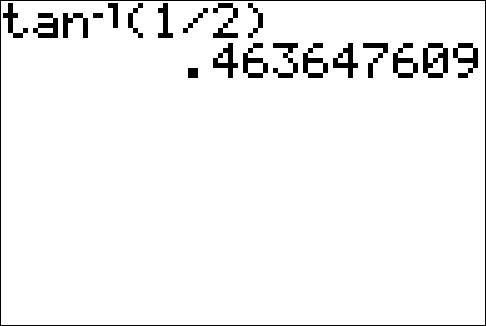
\includegraphics[width=2in]{./IntroTrigGraphics/ArcTrig01.jpg} &
%\hspace{0.75in} 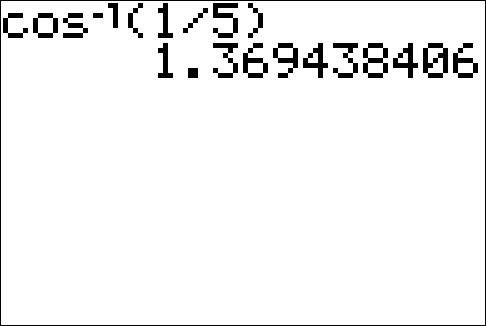
\includegraphics[width=2in]{./IntroTrigGraphics/ArcTrig02.jpg}  \\ 

%\end{tabular} 

\item  Since the argument $-2$ is negative, we cannot directly apply  Theorem \ref{arctangentcotangentfunctionprops} to help us find  $\operatorname{arccot}(-2)$.  Let $t = \operatorname{arccot}(-2)$. Then $t$ is a real number such that $0 < t < \pi$ and $\cot(t) = -2$.  Moreover, since $\cot(t) < 0$, we know $\frac{\pi}{2} < t < \pi$.  Geometrically, this means $t$ corresponds to a Quadrant II angle $\theta = t$ radians.  This allows us to proceed using a `reference angle' approach. Consider $\alpha$, the reference angle for $\theta$, as pictured in Figure \ref{fig:arctrig11}. By definition, $\alpha$ is an acute angle so  $0 < \alpha < \frac{\pi}{2}$, and the Reference Angle Theorem, Theorem \ref{refanglethm}, tells us that $\cot(\alpha) = 2$.  This means  $\alpha = \operatorname{arccot}(2)$ radians.  Since the argument of arccotangent is now a \emph{positive} $2$, we can use  Theorem \ref{arctangentcotangentfunctionprops} to get $\alpha = \operatorname{arccot}(2) =\arctan\left(\frac{1}{2}\right)$ radians. Since $\theta = \pi - \alpha =  \pi - \arctan\left(\frac{1}{2}\right) \approx 2.6779$ radians, we get  $\operatorname{arccot}(-2) \approx 2.6779$.

\mfigure[width=0.95\marginparwidth]{.8}{Evaluating $\operatorname{arccot}(-2)$}{fig:arctrig11}{figures/IntroTrigGraphics/ArcTrig-21}


Another way to attack the problem is to use $\arctan\left(-\frac{1}{2}\right)$.  By definition, the real number $t = \arctan\left(-\frac{1}{2}\right)$ satisfies $\tan(t) = -\frac{1}{2}$ with $-\frac{\pi}{2} < t < \frac{\pi}{2}$.  Since $\tan(t)<0$, we know more specifically that $-\frac{\pi}{2} < t < 0$, so $t$ corresponds to an angle $\beta$ in Quadrant IV.  To find the value of $\operatorname{arccot}(-2)$, we once again visualize the angle $\theta = \operatorname{arccot}(-2)$ radians and note that it is a Quadrant II angle with $\tan(\theta) = -\frac{1}{2}$. (See Figure \ref{fig:arctrig12}.)  This means it is exactly $\pi$ units away from $\beta$, and we get $\theta = \pi + \beta = \pi + \arctan\left(-\frac{1}{2}\right) \approx 2.6779$ radians.  Hence, as before, $\operatorname{arccot}(-2) \approx 2.6779$.

\mfigure[width=0.95\marginparwidth]{.6}{Evaluating $\operatorname{arccot}(-2)$}{fig:arctrig12}{figures/IntroTrigGraphics/ArcTrig-22}

\drawexampleline

\item If the range of arccosecant is taken to be $\left[-\frac{\pi}{2}, 0\right) \cup \left(0, \frac{\pi}{2}\right]$, we can use Theorem \ref{arcsecantcosecantfunctionprops1} to get $\operatorname{arccsc}\left(-\frac{3}{2}\right) = \arcsin\left(-\frac{2}{3}\right) \approx -0.7297$.  If, on the other hand, the range of arccosecant is taken to be $\left(0, \frac{\pi}{2}\right] \cup \left(\pi, \frac{3\pi}{2}\right]$, then we proceed as in the previous problem by  letting $t = \operatorname{arccsc}\left(-\frac{3}{2}\right)$.  Then $t$ is a real number with $\csc(t) = -\frac{3}{2}$.  Since $\csc(t) < 0$, we have that $\pi < \theta \leq \frac{3\pi}{2}$, so $t$ corresponds to a Quadrant III angle, $\theta$, as pictured in Figure \ref{fig:arctrig13}.  As above, we let $\alpha$ be the reference angle for $\theta$.  Then $0 < \alpha < \frac{\pi}{2}$ and $\csc(\alpha) =\frac{3}{2}$, which means $\alpha = \operatorname{arccsc}\left(\frac{3}{2}\right)$ radians.  Since the argument of arccosecant is now positive, we may use Theorem \ref{arcsecantcosecantfunctionprops2}  to get $\alpha = \operatorname{arccsc}\left(\frac{3}{2}\right) = \arcsin\left(\frac{2}{3}\right)$ radians.  Since $\theta = \pi + \alpha = \pi +  \arcsin\left(\frac{2}{3}\right) \approx 3.8713$ radians,  $\operatorname{arccsc}\left(-\frac{3}{2}\right) \approx 3.8713$.

\mfigure[width=0.95\marginparwidth]{.4}{Evaluating $\operatorname{arccsc}\left(-\frac{3}{2}\right)$}{fig:arctrig13}{figures/IntroTrigGraphics/ArcTrig-23}

\end{enumerate}

%\newpage

\item \begin{enumerate}

\item  Since the domain of $F(x) = \arccos(x)$ is $-1 \leq x \leq 1$, we can find the domain of $f(x) = \frac{\pi}{2} - \arccos\left(\frac{x}{5}\right)$ by setting the argument of the arccosine, in this case $\frac{x}{5}$, between $-1$ and $1$. Solving  $-1 \leq \frac{x}{5} \leq 1$ gives $-5 \leq x \leq 5$, so the domain is $[-5,5]$.  To determine the range of $f$, we take a cue from Section \ref{Transformations}. Three `key' points on the graph of $F(x) = \arccos(x)$ are  $(-1, \pi)$, $\left(0, \frac{\pi}{2}\right)$ and $(1,0)$ . Following the procedure outlined in Theorem \ref{transformationsthm}, we track these points to $\left(-5, -\frac{\pi}{2}\right)$, $(0, 0)$ and $\left(5, \frac{\pi}{2}\right)$. Plotting these values tells us that the range of $f$ is $\left[-\frac{\pi}{2}, \frac{\pi}{2}\right]$. (It also confirms our domain!) The graph in Figure \ref{fig:arctrig14} confirms our results.

\mfigure[width=0.95\marginparwidth]{.2}{$y=f(x)=\dfrac{\pi}{2}-\arccos\left(\dfrac{x}{5}\right)$}{fig:arctrig14}{figures/IntroTrigGraphics/ArcTrig1}

\item  To find the domain and range of $f(x) = 3\arctan\left(4x \right)$, we note that since the domain of $F(x) = \arctan(x)$ is all real numbers, the only restrictions, if any, on the domain of  $f(x) = 3\arctan\left(4x \right)$ come from the argument of the arctangent, in this case, $4x$.  Since $4x$ is defined for all real numbers, we have established that the domain of $f$ is all real numbers.  To determine the range of $f$, we can, once again, appeal to Theorem \ref{transformationsthm}.  Choosing our `key' point to be $(0,0)$ and tracking the horizontal asymptotes $y = -\frac{\pi}{2}$ and $y= \frac{\pi}{2}$, we find that the graph of $y = f(x) = 3\arctan\left(4x \right)$ differs from the graph of $y = F(x) = \arctan(x)$ by a horizontal compression by a factor of $4$ and a vertical stretch by a factor of $3$.  It is the latter which affects the range, producing a range of $\left(-\frac{3\pi}{2}, \frac{3\pi}{2} \right)$.  We confirm our findings using GeoGebra in Figure \ref{fig:arctrig15}.

\mfigure[width=0.95\marginparwidth]{.6}{$y=f(x)=3\arctan(4x)$}{fig:arctrig15}{figures/IntroTrigGraphics/ArcTrig2}

\item  To find the domain of $g(x) = \operatorname{arccot}\left(\frac{x}{2}\right) + \pi$, we proceed as above.  Since the domain of $G(x) = \operatorname{arccot}(x)$ is $(-\infty, \infty)$, and $\frac{x}{2}$ is defined for all $x$, we get that the domain of $g$ is $(-\infty, \infty)$ as well.  As for the range, we note that the range of $G(x)  = \operatorname{arccot}(x)$, like that of $F(x) = \arctan(x)$, is limited by a pair of horizontal asymptotes, in this case $y = 0$ and $y = \pi$.  Following  Theorem \ref{transformationsthm}, we graph $y =  g(x) = \operatorname{arccot}\left(\frac{x}{2}\right) + \pi$ starting with $y = G(x) = \operatorname{arccot}(x)$ and first performing a horizontal expansion by a factor of $2$ and following that with a vertical shift upwards by $\pi$.  This latter transformation is the one which affects the range, making it now $(\pi, 2\pi)$.  To check this graphically, we encounter a bit of a problem, since on many calculators, there is no shortcut button corresponding to the arccotangent function. Taking a cue from number \ref{arccotneg2}, we attempt to rewrite $g(x) = \operatorname{arccot}\left(\frac{x}{2}\right) + \pi$ in terms of the arctangent function. Using Theorem \ref{arctangentcotangentfunctionprops}, we have that $\operatorname{arccot}\left(\frac{x}{2}\right) = \arctan\left(\frac{2}{x}\right)$ when $\frac{x}{2} > 0$, or, in this case, when $x > 0$.  Hence, for $x > 0$, we have $g(x) = \arctan\left(\frac{2}{x}\right) + \pi$.  When $\frac{x}{2} < 0$, we can use the same argument in number \ref{arccotneg2} that gave us $\operatorname{arccot}(-2) = \pi + \arctan\left(-\frac{1}{2}\right)$ to give us $\operatorname{arccot}\left(\frac{x}{2}\right) = \pi + \arctan\left(\frac{2}{x}\right)$.  Hence, for $x < 0$, $g(x) = \pi + \arctan\left(\frac{2}{x}\right) + \pi = \arctan\left(\frac{2}{x}\right) + 2\pi$.  What about $x=0$?  We know $g(0) = \operatorname{arccot}(0) + \pi = \pi$, and neither of the formulas for $g$ involving arctangent will produce this result. Hence, in order to graph $y = g(x)$ on our computer or calculator, we need to write it as a piecewise defined function:

\[ g(x) = \operatorname{arccot}\left(\frac{x}{2}\right) + \pi = \left\{ \begin{array}{rr} \arctan\left(\frac{2}{x}\right) + 2\pi, & \text{if $x<0$} \\ [5pt] \pi, & \text{if $x=0$} \\ [5pt] \arctan\left(\frac{2}{x}\right) + \pi, & \text{if $x>0$} \end{array}\right. \]

The result is shown in Figure \ref{fig:arctrig16}.

\mfigure[width=0.95\marginparwidth]{.4}{$y=g(x)=\operatorname{arccot}\left(\dfrac{\pi}{2}\right)+\pi$}{fig:arctrig16}{figures/IntroTrigGraphics/ArcTrig3}

\mnote{.2}{Note: as with a graphing calculator, the GeoGebra software does not have an arccotangent function. To input a piecewise-defined function in GeoGebra, we use the syntax \texttt{Function[<function>, <start x value>, <end x value>.]}.}

\smallskip

\end{enumerate}

\end{enumerate}
}



\medskip


The inverse trigonometric functions are typically found in applications whenever the measure of an angle is required.  One such scenario is presented in the following example. (The authors would like to thank Dan Stitz for this problem and associated graphics.)

\pagebreak

\example{roofpitchex}{Angle of a pitched roof}{  The roof on the house below has a  `$6/12$ pitch'.  This means that when viewed from the side, the roof line has a rise of 6 feet over a run of 12 feet.  Find the angle of inclination from the bottom of the roof to the top of the roof.  Express your answer in decimal degrees, rounded to the nearest hundredth of a degree.

\medskip

\noindent\begin{minipage}{\textwidth}
\begin{center}
\begin{tabular}{cc}
\myincludegraphics[width=0.5\textwidth]{figures/IntroTrigGraphics/ArcTrig05}&
\myincludegraphics[width=0.4\textwidth]{figures/IntroTrigGraphics/ArcTrig06}\\
Front View & Side View
\end{tabular}
\end{center}
\end{minipage}
}
{
If we divide the side view of the house down the middle, we find that the roof line forms the hypotenuse of a right triangle with legs of length $6$ feet and $12$ feet.  Using Theorem \ref{circularfunctionstriangle}, we find the angle of inclination, labelled $\theta$ in Figure \ref{fig:arctrigappex}, satisfies $\tan(\theta) = \frac{6}{12} = \frac{1}{2}$.  Since $\theta$ is an acute angle, we can use the arctangent function and we find $\theta = \arctan\left(\frac{1}{2}\right)\, \text{radians} \, \approx 26.56^{\circ}$.

\mfigure[width=0.95\marginparwidth]{.65}{Angle of inclination $\theta$ for Example \ref{roofpitchex}}{fig:arctrigappex}{figures/IntroTrigGraphics/ArcTrig-24}
}



\medskip

\subsection{Solving Equations Using the Inverse Trigonometric Functions.}

In Sections \ref{TheUnitCircle} and \ref{CircularFunctions}, we learned how to solve equations like $\sin(\theta) = \frac{1}{2}$ for angles $\theta$ and $\tan(t) = -1$ for real numbers $t$. In each case, we ultimately appealed to the Unit Circle and relied on the fact that the answers corresponded to a set of `common angles' listed on page \pageref{commonanglesunitcircle}.  If, on the other hand, we had been asked to find all angles with $\sin(\theta) = \frac{1}{3}$ or solve $\tan(t) = -2$ for real numbers $t$, we would have been hard-pressed to do so.  With the introduction of the inverse trigonometric functions, however, we are now in a position to solve these equations. A good parallel to keep in mind is how the square root function can be used to solve certain quadratic equations.  The equation $x^2 = 4$ is a lot like  $\sin(\theta) = \frac{1}{2}$ in that it has friendly, `common value' answers  $x = \pm 2$.  The equation $x^2 = 7$, on the other hand, is a lot like $\sin(\theta) = \frac{1}{3}$.  We know there are answers (how do we know this again?), but we can't express them using `friendly' numbers. (This is all, of course, a matter of opinion.  For the record, the authors find $\pm \sqrt{7}$ just as `nice' as $\pm 2$.)  To solve $x^2 = 7$, we make use of the square root function and write $x = \pm \sqrt{7}$. We can certainly \textit{approximate} these answers using a calculator, but as far as exact answers go, we leave them as $x = \pm \sqrt{7}$.  In the same way, we will use the arcsine function to solve $\sin(\theta) = \frac{1}{3}$, as seen in the following example.

\pagebreak

\example{basicinverseeqns}{Solving trigonometric equations}{  Solve the following equations.

\begin{enumerate}

\item  \label{basicinverseeqnssine} Find all angles $\theta$ for which $\sin(\theta) = \frac{1}{3}$.

\item \label{basicinverseeqnstangent} Find all real numbers $t$ for which $\tan(t) = -2$

\item  \label{basicinverseeqnssecant} Solve $\, \sec(x) = -\frac{5}{3} \,$ for $x$.

\end{enumerate}
}
{
\begin{enumerate}

\item  If $\sin(\theta) = \frac{1}{3}$, then the terminal side of $\theta$, when plotted in standard position, intersects the Unit Circle at $y = \frac{1}{3}$.  Geometrically, we see that this happens at two places:  in Quadrant I and Quadrant II. If we let $\alpha$ denote the acute solution to the equation, then all the solutions to this equation in Quadrant I  are coterminal with $\alpha$, and $\alpha$ serves as the reference angle for all of the solutions to this equation in Quadrant II.

\mtable{.7}{Solving $\sin(\theta)=\frac{1}{3}$}{fig:trigeqn1}{
\begin{tabular}{c}
\myincludegraphics[width=0.95\marginparwidth]{figures/IntroTrigGraphics/ArcTrig-25}\\
\\
\myincludegraphics[width=0.95\marginparwidth]{figures/IntroTrigGraphics/ArcTrig-26}
\end{tabular}}

Since $\frac{1}{3}$ isn't the sine of any of the `common angles' discussed earlier, we use the arcsine functions to express our answers.  The real number $t = \arcsin\left(\frac{1}{3}\right)$ is defined so it satisfies $0 < t < \frac{\pi}{2}$ with $\sin(t) = \frac{1}{3}$.  Hence, $\alpha = \arcsin\left(\frac{1}{3}\right)$ radians. Since the solutions in Quadrant I are all coterminal with $\alpha$, we get part of our solution to be $\theta = \alpha + 2\pi k  = \arcsin\left(\frac{1}{3}\right) + 2\pi k$ for integers $k$.  Turning our attention to Quadrant II, we get one solution to be $\pi - \alpha$.  Hence, the Quadrant II solutions are  $\theta = \pi - \alpha + 2\pi k = \pi - \arcsin\left(\frac{1}{3}\right) + 2\pi k$, for integers $k$.


\item We may visualize the solutions to $\tan(t)=-2$ as angles $\theta$  with $\tan(\theta) = -2$.  Since tangent is negative only in Quadrants II and IV, we focus our efforts there. 



\mtable{.3}{Solving $\tan(t)=-2$}{fig:trigeqn2}{
\begin{tabular}{c}
\myincludegraphics[width=0.95\marginparwidth]{figures/IntroTrigGraphics/ArcTrig-27}\\
\\
\myincludegraphics[width=0.95\marginparwidth]{figures/IntroTrigGraphics/ArcTrig-28}
\end{tabular}}

Since $-2$ isn't the tangent of any of the `common angles', we need to use the arctangent function to express our answers.  The real number $t = \arctan(-2)$ satisfies $\tan(t)=-2$  and $-\frac{\pi}{2} < t < 0$.   If we let $\beta = \arctan(-2)$ radians, we see that all of the Quadrant IV solutions to  $\tan(\theta) = -2$  are coterminal with $\beta$. Moreover, the solutions from Quadrant II differ by exactly $\pi$ units from the solutions in Quadrant IV, so all the solutions to $\tan(\theta) = -2$ are of the form $\theta = \beta + \pi k = \arctan(-2) + \pi k$ for some integer $k$.  Switching back to the variable $t$,  we record our final answer to $\tan(t) = -2$ as $t = \arctan(-2) + \pi k$ for integers $k$.


\item  The last equation we are asked to solve, $\sec(x) = -\frac{5}{3}$, poses two immediate problems.  First, we are not told whether or not $x$ represents an angle or a real number.  We assume the latter, but note that we will use angles and the Unit Circle to solve the equation regardless.  Second, as we have mentioned, there is no universally accepted range of the arcsecant function.  For that reason, we adopt the advice given in Section \ref{CircularFunctions} and convert this to the cosine problem $\cos(x) = -\frac{3}{5}$.  Adopting an angle approach, we consider the equation $\cos(\theta) = -\frac{3}{5}$ and note that our solutions lie in Quadrants II and III.  Since $-\frac{3}{5}$ isn't  the cosine of any of the `common angles', we'll need to express our solutions in terms of the arccosine function.  The real number $t = \arccos\left(-\frac{3}{5}\right)$ is defined so that $\frac{\pi}{2} < t < \pi$ with $\cos(t) = -\frac{3}{5}$.  If we let $\beta = \arccos\left(-\frac{3}{5}\right)$ radians, we see that $\beta$ is a Quadrant II angle.  To obtain a Quadrant III angle solution, we may simply use $-\beta = -\arccos\left(-\frac{3}{5}\right)$.  Since all angle solutions are coterminal with $\beta$ or $-\beta$, we get our solutions to $\cos(\theta) = -\frac{3}{5}$ to be $\theta = \beta + 2\pi k = \arccos\left(-\frac{3}{5}\right) + 2\pi k$ or $\theta = -\beta + 2\pi k = -\arccos\left(-\frac{3}{5}\right) + 2\pi k$ for integers $k$.  Switching back to the variable $x$,  we record our final answer to $\sec(x) = -\frac{5}{3}$ as $x = \arccos\left(-\frac{3}{5}\right) + 2\pi k$ or $x = -\arccos\left(-\frac{3}{5}\right) + 2\pi k$ for integers $k$.


\medskip

\mtable{.7}{Solving $\sec(x)=-\frac{5}{3}$}{fig:trigeqn3}{
\begin{tabular}{c}
\myincludegraphics[width=0.95\marginparwidth]{figures/IntroTrigGraphics/ArcTrig-29}\\
\\
\myincludegraphics[width=0.95\marginparwidth]{figures/IntroTrigGraphics/ArcTrig-30}
\end{tabular}}

\end{enumerate}
}

\medskip

 The reader is encouraged to check the answers found in Example \ref{basicinverseeqns} - both analytically and with the calculator (see Section \ref{sectionarcstuffoncalc}).  With practice, the inverse trigonometric functions will become as familiar to you as the square root function.  Speaking of practice \dots


\printexercises{exercises_pre/07_06_exercises}